% Options for packages loaded elsewhere
\PassOptionsToPackage{unicode}{hyperref}
\PassOptionsToPackage{hyphens}{url}
\PassOptionsToPackage{dvipsnames,svgnames,x11names}{xcolor}
%
\documentclass[
]{report}

\usepackage{amsmath,amssymb}
\usepackage{iftex}
\ifPDFTeX
  \usepackage[T1]{fontenc}
  \usepackage[utf8]{inputenc}
  \usepackage{textcomp} % provide euro and other symbols
\else % if luatex or xetex
  \usepackage{unicode-math}
  \defaultfontfeatures{Scale=MatchLowercase}
  \defaultfontfeatures[\rmfamily]{Ligatures=TeX,Scale=1}
\fi
\usepackage{lmodern}
\ifPDFTeX\else  
    % xetex/luatex font selection
\fi
% Use upquote if available, for straight quotes in verbatim environments
\IfFileExists{upquote.sty}{\usepackage{upquote}}{}
\IfFileExists{microtype.sty}{% use microtype if available
  \usepackage[]{microtype}
  \UseMicrotypeSet[protrusion]{basicmath} % disable protrusion for tt fonts
}{}
\makeatletter
\@ifundefined{KOMAClassName}{% if non-KOMA class
  \IfFileExists{parskip.sty}{%
    \usepackage{parskip}
  }{% else
    \setlength{\parindent}{0pt}
    \setlength{\parskip}{6pt plus 2pt minus 1pt}}
}{% if KOMA class
  \KOMAoptions{parskip=half}}
\makeatother
\usepackage{xcolor}
\setlength{\emergencystretch}{3em} % prevent overfull lines
\setcounter{secnumdepth}{-\maxdimen} % remove section numbering
% Make \paragraph and \subparagraph free-standing
\ifx\paragraph\undefined\else
  \let\oldparagraph\paragraph
  \renewcommand{\paragraph}[1]{\oldparagraph{#1}\mbox{}}
\fi
\ifx\subparagraph\undefined\else
  \let\oldsubparagraph\subparagraph
  \renewcommand{\subparagraph}[1]{\oldsubparagraph{#1}\mbox{}}
\fi

\usepackage{color}
\usepackage{fancyvrb}
\newcommand{\VerbBar}{|}
\newcommand{\VERB}{\Verb[commandchars=\\\{\}]}
\DefineVerbatimEnvironment{Highlighting}{Verbatim}{commandchars=\\\{\}}
% Add ',fontsize=\small' for more characters per line
\usepackage{framed}
\definecolor{shadecolor}{RGB}{241,243,245}
\newenvironment{Shaded}{\begin{snugshade}}{\end{snugshade}}
\newcommand{\AlertTok}[1]{\textcolor[rgb]{0.68,0.00,0.00}{#1}}
\newcommand{\AnnotationTok}[1]{\textcolor[rgb]{0.37,0.37,0.37}{#1}}
\newcommand{\AttributeTok}[1]{\textcolor[rgb]{0.40,0.45,0.13}{#1}}
\newcommand{\BaseNTok}[1]{\textcolor[rgb]{0.68,0.00,0.00}{#1}}
\newcommand{\BuiltInTok}[1]{\textcolor[rgb]{0.00,0.23,0.31}{#1}}
\newcommand{\CharTok}[1]{\textcolor[rgb]{0.13,0.47,0.30}{#1}}
\newcommand{\CommentTok}[1]{\textcolor[rgb]{0.37,0.37,0.37}{#1}}
\newcommand{\CommentVarTok}[1]{\textcolor[rgb]{0.37,0.37,0.37}{\textit{#1}}}
\newcommand{\ConstantTok}[1]{\textcolor[rgb]{0.56,0.35,0.01}{#1}}
\newcommand{\ControlFlowTok}[1]{\textcolor[rgb]{0.00,0.23,0.31}{#1}}
\newcommand{\DataTypeTok}[1]{\textcolor[rgb]{0.68,0.00,0.00}{#1}}
\newcommand{\DecValTok}[1]{\textcolor[rgb]{0.68,0.00,0.00}{#1}}
\newcommand{\DocumentationTok}[1]{\textcolor[rgb]{0.37,0.37,0.37}{\textit{#1}}}
\newcommand{\ErrorTok}[1]{\textcolor[rgb]{0.68,0.00,0.00}{#1}}
\newcommand{\ExtensionTok}[1]{\textcolor[rgb]{0.00,0.23,0.31}{#1}}
\newcommand{\FloatTok}[1]{\textcolor[rgb]{0.68,0.00,0.00}{#1}}
\newcommand{\FunctionTok}[1]{\textcolor[rgb]{0.28,0.35,0.67}{#1}}
\newcommand{\ImportTok}[1]{\textcolor[rgb]{0.00,0.46,0.62}{#1}}
\newcommand{\InformationTok}[1]{\textcolor[rgb]{0.37,0.37,0.37}{#1}}
\newcommand{\KeywordTok}[1]{\textcolor[rgb]{0.00,0.23,0.31}{#1}}
\newcommand{\NormalTok}[1]{\textcolor[rgb]{0.00,0.23,0.31}{#1}}
\newcommand{\OperatorTok}[1]{\textcolor[rgb]{0.37,0.37,0.37}{#1}}
\newcommand{\OtherTok}[1]{\textcolor[rgb]{0.00,0.23,0.31}{#1}}
\newcommand{\PreprocessorTok}[1]{\textcolor[rgb]{0.68,0.00,0.00}{#1}}
\newcommand{\RegionMarkerTok}[1]{\textcolor[rgb]{0.00,0.23,0.31}{#1}}
\newcommand{\SpecialCharTok}[1]{\textcolor[rgb]{0.37,0.37,0.37}{#1}}
\newcommand{\SpecialStringTok}[1]{\textcolor[rgb]{0.13,0.47,0.30}{#1}}
\newcommand{\StringTok}[1]{\textcolor[rgb]{0.13,0.47,0.30}{#1}}
\newcommand{\VariableTok}[1]{\textcolor[rgb]{0.07,0.07,0.07}{#1}}
\newcommand{\VerbatimStringTok}[1]{\textcolor[rgb]{0.13,0.47,0.30}{#1}}
\newcommand{\WarningTok}[1]{\textcolor[rgb]{0.37,0.37,0.37}{\textit{#1}}}

\providecommand{\tightlist}{%
  \setlength{\itemsep}{0pt}\setlength{\parskip}{0pt}}\usepackage{longtable,booktabs,array}
\usepackage{calc} % for calculating minipage widths
% Correct order of tables after \paragraph or \subparagraph
\usepackage{etoolbox}
\makeatletter
\patchcmd\longtable{\par}{\if@noskipsec\mbox{}\fi\par}{}{}
\makeatother
% Allow footnotes in longtable head/foot
\IfFileExists{footnotehyper.sty}{\usepackage{footnotehyper}}{\usepackage{footnote}}
\makesavenoteenv{longtable}
\usepackage{graphicx}
\makeatletter
\def\maxwidth{\ifdim\Gin@nat@width>\linewidth\linewidth\else\Gin@nat@width\fi}
\def\maxheight{\ifdim\Gin@nat@height>\textheight\textheight\else\Gin@nat@height\fi}
\makeatother
% Scale images if necessary, so that they will not overflow the page
% margins by default, and it is still possible to overwrite the defaults
% using explicit options in \includegraphics[width, height, ...]{}
\setkeys{Gin}{width=\maxwidth,height=\maxheight,keepaspectratio}
% Set default figure placement to htbp
\makeatletter
\def\fps@figure{htbp}
\makeatother

\usepackage{booktabs}
\usepackage{amsthm}
\usepackage{placeins}
\makeatletter
\def\thm@space@setup{%
  \thm@preskip=8pt plus 2pt minus 4pt
  \thm@postskip=\thm@preskip
}
\makeatother
\usepackage{adjustbox}
\usepackage{awesomebox}
\usepackage{color}
\usepackage{framed}
\setlength{\fboxsep}{.8em}
\usepackage[most]{tcolorbox}
\usepackage{blindtext}
\usepackage{amsmath}
\usepackage{amssymb}
\usepackage{bm}
\usepackage[finnish]{babel}
\usepackage{graphicx}
\usepackage{placeins}
\usepackage{overpic}
\usepackage{lmodern}
\usepackage{epsfig}
\usepackage{placeins}
\usepackage{xstring}     % Used for \IfEqCase


\definecolor{myboxcolor}{named}{blue} % Default box color

\definecolor{my-purple}{RGB}{204,180,225}
\newtcolorbox{defblock}[1]{%
    breakable,
    enhanced,
    coltext=black,
    colback=my-purple,      % Box color is used here
    colframe=myboxcolor!25!my-purple,     % Box color is used here
    detach title,
    after upper={\par\hfill\tcbtitle}        % Box title is used here 
}

\definecolor{my-orange}{RGB}{255,205,138}
\newtcolorbox{eblock}[1]{%
    breakable,
    enhanced,
    coltext=black,
    colback=my-orange,      % Box color is used here
    colframe=myboxcolor!25!my-orange,     % Box color is used here
    detach title,
    after upper={\par\hfill\tcbtitle}        % Box title is used here 
}


\newcommand{\Rspace}{\mathcal{R}}

\newcommand{\N}{\mathsf{N}}
\newcommand{\Cov}{\mathsf{Cov}}

\newcommand{\Prob}{\mathsf{P}}

\newcommand{\X}{\textbf{X}} 
\newcommand{\Y}{\textbf{Y}} 
\newcommand{\x}{\textbf{x}}                                   
\newcommand{\y}{\textbf{y}}  
\newcommand{\boldc}{\textbf{c}} 
\newcommand{\boldd}{\textbf{d}}  
\newcommand{\bolda}{\textbf{a}}  
\newcommand{\THETA}{\mx{\theta}}
\newcommand{\PHI}{\mx{\phi}}                                   
\newcommand{\VAREPSILON}{\mx{\varepsilon}}                                   
\newcommand{\hatVAREPSILON}{\mx{\hat{\VAREPSILON}}}
\newcommand{\boldP}{\textbf{P}}
\newcommand{\boldM}{\textbf{M}}
\newcommand{\z}{\mx{z}}
\newcommand{\A}{\textbf{A}}
\newcommand{\C}{\textbf{C}}
\newcommand{\hatMU}{\mx{\hat{\mu}}}
\newcommand{\SIGMA}{\mx{\Sigma}}
\newcommand{\ZERO}{\mx{0}}
\newcommand{\ONE}{\mx{1}}
\newcommand{\diag}{\textbf{I}}

\newcommand{\bl}[1]{\textcolor{blue}{#1}}
\newcommand{\rd}[1]{\textcolor{red}{#1}}
\newcommand{\gr}[1]{\textcolor{darkgreenx}{#1}}


%\newcommand\indep{\protect\mathpalette{\protect\independenT}{\perp}}
%\def\independenT#1#2{\mathrel{\rlap{$#1#2$}\mkern2mu{#1#2}}}
\makeatletter
\makeatother
\makeatletter
\makeatother
\makeatletter
\@ifpackageloaded{caption}{}{\usepackage{caption}}
\AtBeginDocument{%
\ifdefined\contentsname
  \renewcommand*\contentsname{Table of contents}
\else
  \newcommand\contentsname{Table of contents}
\fi
\ifdefined\listfigurename
  \renewcommand*\listfigurename{List of Figures}
\else
  \newcommand\listfigurename{List of Figures}
\fi
\ifdefined\listtablename
  \renewcommand*\listtablename{List of Tables}
\else
  \newcommand\listtablename{List of Tables}
\fi
\ifdefined\figurename
  \renewcommand*\figurename{Figure}
\else
  \newcommand\figurename{Figure}
\fi
\ifdefined\tablename
  \renewcommand*\tablename{Table}
\else
  \newcommand\tablename{Table}
\fi
}
\@ifpackageloaded{float}{}{\usepackage{float}}
\floatstyle{ruled}
\@ifundefined{c@chapter}{\newfloat{codelisting}{h}{lop}}{\newfloat{codelisting}{h}{lop}[chapter]}
\floatname{codelisting}{Listing}
\newcommand*\listoflistings{\listof{codelisting}{List of Listings}}
\makeatother
\makeatletter
\@ifpackageloaded{caption}{}{\usepackage{caption}}
\@ifpackageloaded{subcaption}{}{\usepackage{subcaption}}
\makeatother
\makeatletter
\@ifpackageloaded{tcolorbox}{}{\usepackage[skins,breakable]{tcolorbox}}
\makeatother
\makeatletter
\@ifundefined{shadecolor}{\definecolor{shadecolor}{rgb}{.97, .97, .97}}
\makeatother
\makeatletter
\makeatother
\makeatletter
\makeatother
\ifLuaTeX
  \usepackage{selnolig}  % disable illegal ligatures
\fi
\IfFileExists{bookmark.sty}{\usepackage{bookmark}}{\usepackage{hyperref}}
\IfFileExists{xurl.sty}{\usepackage{xurl}}{} % add URL line breaks if available
\urlstyle{same} % disable monospaced font for URLs
\hypersetup{
  pdftitle={Luku 7 - Tilastollinen riippuvuus ja korrelaatio},
  colorlinks=true,
  linkcolor={blue},
  filecolor={Maroon},
  citecolor={Blue},
  urlcolor={Blue},
  pdfcreator={LaTeX via pandoc}}

\title{Luku 7 - Tilastollinen riippuvuus ja korrelaatio}
\usepackage{etoolbox}
\makeatletter
\providecommand{\subtitle}[1]{% add subtitle to \maketitle
  \apptocmd{\@title}{\par {\large #1 \par}}{}{}
}
\makeatother
\subtitle{Tiivistelmä}
\author{}
\date{}

\begin{document}
\maketitle
\ifdefined\Shaded\renewenvironment{Shaded}{\begin{tcolorbox}[boxrule=0pt, sharp corners, frame hidden, enhanced, interior hidden, breakable, borderline west={3pt}{0pt}{shadecolor}]}{\end{tcolorbox}}\fi

\hypertarget{luvun-ydinviesti}{%
\section{Luvun ydinviesti}\label{luvun-ydinviesti}}

Tähän mennessä kurssilla käsitellyt tilastolliset tunnusluvut ja niihin
perustuva päättely (luku 6) on keskittynyt yhden tilastollisen muuttujan
havaittujen arvojen tutkimiseen.

Kuten aiemmista luvuista kuitenkin tiedetään, niin usein tutkimuksen
mielenkiinnon kohteena on useammat tilastoyksikön tilastolliset
muuttujat.

Tässä luvussa tarkastellaan tilastollisia tutkimusasetelmia, joissa on
mukana kaksi tai useampia muuttujia. Erityisesti tarkastellaan sitä,
miten kahden tai useamman muuttujan samanaikainen tarkastelu vaikuttaa
tilastolliseen analyysiin.

Keskeistä on erottaa toisistaan tilastollinen riippuvuus ja eksakti
riippuvuus sekä korrelaatio ja kausaalisuus!

\hypertarget{muuttujien-vuxe4liset-riippuvuudet}{%
\section{Muuttujien väliset
riippuvuudet}\label{muuttujien-vuxe4liset-riippuvuudet}}

Tieteellisen tutkimuksen tärkeimmät ja mielenkiintoisimmat kysymykset
liittyvät tavallisesti \textbf{tutkimuksen kohteena olevaa ilmiötä
kuvaavien muuttujien välisiin riippuvuuksiin.}

Tällöin tarvitaan menetelmiä, jotka mahdollistavat kahden tai useamman
muuttujan välisten riippuvuuksien kuvaamisen ja mallintamisen. Tärkeää
on kuitenkin erottaa muuttujien \textbf{eksakti} ja
\textbf{tilastollinen riippuvuus.}

\begin{itemize}
\item
  \textbf{Eksakti riippuvuus} on sellaista riippuvuutta, joka
  mahdollistaa yhden muuttujan arvojen tarkan (täydellisen) ennustamisen
  kun tiedetään toisen muuttujan saamat arvot.
\item
  \textbf{Tilastollinen riippuvuus} on sellaista riippuvuutta, jossa
  muuttujien välillä ei ole eksaktia riippuvuutta, mutta toisen
  muuttujan arvoja voidaan käyttää apuna toisen muuttujan arvojen
  mallintamisesssa ja mahdollisesti myös ennustamisessa.
\end{itemize}

\hypertarget{kahden-muuttujan-havaintoaineiston-kuvaaminen}{%
\section{Kahden muuttujan havaintoaineiston
kuvaaminen}\label{kahden-muuttujan-havaintoaineiston-kuvaaminen}}

Samoin kuin yhden muuttujan tapauksessa, lähtökohta kahden tai useamman
muuttujan havaintoaineistojen kuvaamiselle on tutustua niiden jakaumaan.

\begin{itemize}
\item
  \textbf{Graafiset esitykset} kuvaavat ja esittelevät
  havaintoaineistojen jakaumaa kokonaisuuten erilaisten kuvaajien
  avulla.

  \begin{itemize}
  \item
    Usein mielekästä vain kaksiulotteisten kuvaajien avulla, joten
    useampiulotteisia aineistoja kuvataan usein kahden muuttujan välisin
    kuvaajin.
  \item
    \textbf{Kahden järjestys-, välimatka- tai suhdeasteikollisen
    muuttujan havaittujen arvojen pareja havainnollistetaan tavallisesti
    hajontakuviolla eli pistediagrammilla} (engl. scatter plot).
  \end{itemize}
\end{itemize}

\begin{itemize}
\item
  \textbf{Otostunnusluvut} kuvaavat havaintoaineistojen jakauman
  ominaisuuksia tilastollisin tunnusluvuin.

  \begin{itemize}
  \tightlist
  \item
    Muuttujakohtaiset otostunnusluvut, kuten otoskeskiarvo tai
    otosvarianssi (ks. luku 6), eivät kuitenkaan kerro mitään muuttujien
    välisestä riippuvuudesta! \textbf{Tarvitaan siis tilastollista
    riippuvuutta kuvaavia otostunnuslukuja}.
  \end{itemize}
\end{itemize}

\hypertarget{pistediagrammi}{%
\section{Pistediagrammi}\label{pistediagrammi}}

\begin{defblock}{}
\textbf{Pistediagrammi}

Olkoot \(X\) ja \(Y\) järjestys-, välimatka- tai suhdeasteikollisia
muuttujia, joiden havaitut arvot ovat \(x_1, x_2,\dots,x_n\) ja
\(y_1,y_2,\dots,y_n\). Oletetaan lisäksi, että havaintoarvot \(x_i\) ja
\(y_i\) liittyvät samaan havaintoyksikköön kaikille \(i=1,2,\dots,n\).
Havaintoarvojen parien \((x_i,y_i)\) pistediagrammi saadaan esittämällä
lukuparit niiden määrittelemien pisteiden tasokoordinaatistossa.

\end{defblock}

\begin{figure}

{\centering 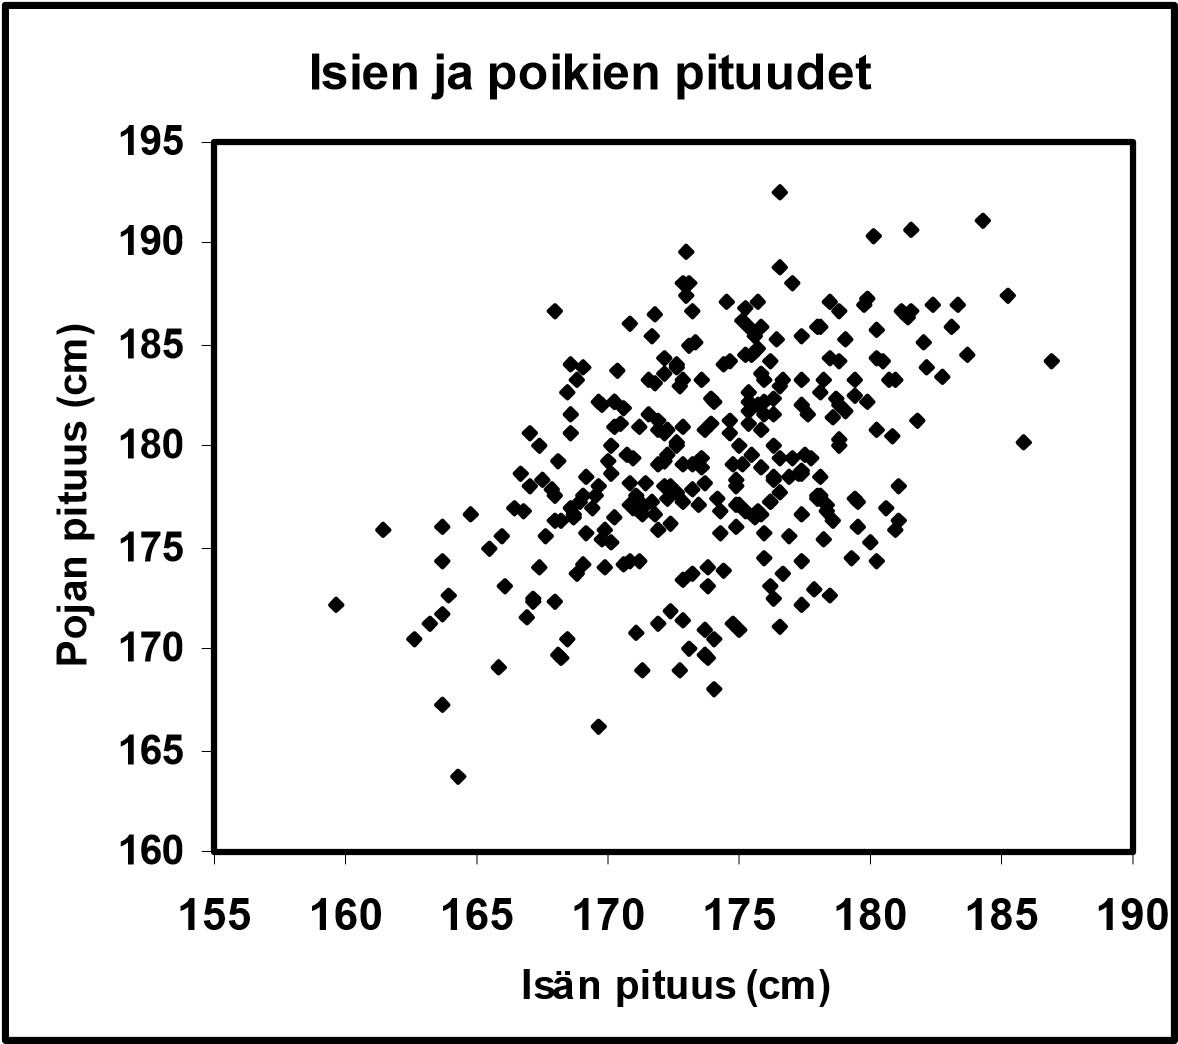
\includegraphics[width=4.84375in,height=\textheight]{images/Isien-poikien-pituudet-Mellin.jpg}

}

\caption{Isien ja poikien pituudet. Lähde: Mellin (2006).}

\end{figure}

\hypertarget{tunnusluvut}{%
\section{Tunnusluvut}\label{tunnusluvut}}

Kahden välimatka- tai suhdeasteikollisen muuttujan havaintoarvjen parien
muodostamaa jakaumaa voidaan karakterisoida jo tunnetuilla keskiarvoilla
(jakaumien keskimääräiset sijainnit) sekä otosvariansseilla (jakaumien
hajonta).

\begin{itemize}
\tightlist
\item
  Nämä eivät kuitenkaan kuvaa muuttujien välistä (lineaarista)
  riippuvuutta!
\end{itemize}

Kahden satunnaismuuttujan \(X\) ja \(Y\) havaittujen arvojen
\(x_1,x_2,\dots,x_n\) ja \(y_1, y_2,\dots,y_n\) muodostamista pareista
\((x_i, y_i)\) (havaitut arvot liittyvät samaan havaintoyksikköön
\(i=1,2,\dots,n\)) voidaan laskea muuttujakohtaiset otoskeskiarvot
\(\bar{x} = \frac{1}{n}\sum_{i=1}^n y_i\) ja
\(\bar{y} = \frac{1}{n}\sum_{i=1}^n y_i\).

Koska \(\bar{x}\) kuvaa satunnaismuuttujan \(X\) havaittujen arvojen
painopistettä ja \(\bar{y}\) kuvaa satunnaismuuttujan \(Y\)
painopistettä, niin lukupari \((\bar{x},\bar{y})\) on havaintoarvojen
parien muodostamien pisteiden painopiste.

\hypertarget{tunnusluvut-riippumaton-tapaus}{%
\section{Tunnusluvut: riippumaton
tapaus}\label{tunnusluvut-riippumaton-tapaus}}

\begin{Shaded}
\begin{Highlighting}[]
\NormalTok{plotdata }\OtherTok{=} \FunctionTok{data.frame}\NormalTok{(MASS}\SpecialCharTok{::}\FunctionTok{mvrnorm}\NormalTok{(}\AttributeTok{n =} \DecValTok{1000}\NormalTok{, }\AttributeTok{mu =} \FunctionTok{c}\NormalTok{(}\DecValTok{150}\NormalTok{, }\DecValTok{180}\NormalTok{), }\AttributeTok{Sigma =} \FunctionTok{matrix}\NormalTok{(}\FunctionTok{c}\NormalTok{(}\DecValTok{15}\NormalTok{, }\DecValTok{0}\NormalTok{, }\DecValTok{0}\NormalTok{, }\DecValTok{15}\NormalTok{), }\AttributeTok{nrow =} \DecValTok{2}\NormalTok{, }\AttributeTok{byrow =}\NormalTok{ T)))}
\FunctionTok{theme\_set}\NormalTok{(}\FunctionTok{theme\_bw}\NormalTok{())}
\NormalTok{ggplot2}\SpecialCharTok{::}\FunctionTok{ggplot}\NormalTok{(plotdata) }\SpecialCharTok{+}\NormalTok{ ggplot2}\SpecialCharTok{::}\FunctionTok{geom\_point}\NormalTok{(}\FunctionTok{aes}\NormalTok{(}\AttributeTok{x =}\NormalTok{ X1, }\AttributeTok{y =}\NormalTok{ X2)) }\SpecialCharTok{+} \FunctionTok{xlab}\NormalTok{(}\StringTok{"Muuttujan X havaitut arvot x"}\NormalTok{) }\SpecialCharTok{+} \FunctionTok{ylab}\NormalTok{(}\StringTok{"Muuttujan Y havaitut arvot y"}\NormalTok{)}
\end{Highlighting}
\end{Shaded}

\begin{figure}[H]

{\centering 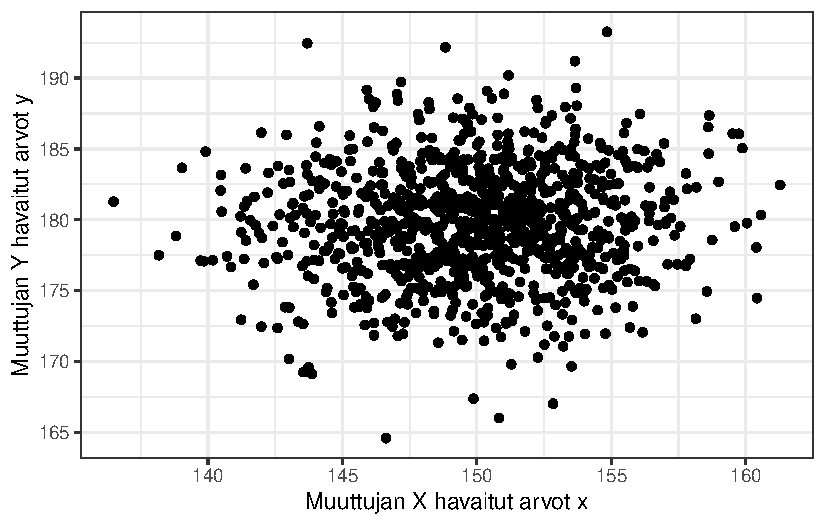
\includegraphics{Tiivistelma6_files/figure-pdf/unnamed-chunk-2-1.pdf}

}

\end{figure}

\hypertarget{tunnusluvut-muuttujat-riippuvaisia}{%
\section{Tunnusluvut: muuttujat
riippuvaisia}\label{tunnusluvut-muuttujat-riippuvaisia}}

\begin{Shaded}
\begin{Highlighting}[]
\NormalTok{plotdata }\OtherTok{=} \FunctionTok{data.frame}\NormalTok{(MASS}\SpecialCharTok{::}\FunctionTok{mvrnorm}\NormalTok{(}\AttributeTok{n =} \DecValTok{1000}\NormalTok{, }\AttributeTok{mu =} \FunctionTok{c}\NormalTok{(}\DecValTok{150}\NormalTok{, }\DecValTok{180}\NormalTok{), }\AttributeTok{Sigma =} \FunctionTok{matrix}\NormalTok{(}\FunctionTok{c}\NormalTok{(}\DecValTok{15}\NormalTok{, }\DecValTok{10}\NormalTok{, }\DecValTok{10}\NormalTok{, }\DecValTok{15}\NormalTok{), }\AttributeTok{nrow =} \DecValTok{2}\NormalTok{, }\AttributeTok{byrow =}\NormalTok{ T)))}
\NormalTok{ggplot2}\SpecialCharTok{::}\FunctionTok{ggplot}\NormalTok{(plotdata) }\SpecialCharTok{+}\NormalTok{ ggplot2}\SpecialCharTok{::}\FunctionTok{geom\_point}\NormalTok{(}\FunctionTok{aes}\NormalTok{(}\AttributeTok{x =}\NormalTok{ X1, }\AttributeTok{y =}\NormalTok{ X2)) }\SpecialCharTok{+} \FunctionTok{xlab}\NormalTok{(}\StringTok{"Muuttujan X havaitut arvot x"}\NormalTok{) }\SpecialCharTok{+} \FunctionTok{ylab}\NormalTok{(}\StringTok{"Muuttujan Y havaitut arvot y"}\NormalTok{)}
\end{Highlighting}
\end{Shaded}

\begin{figure}[H]

{\centering 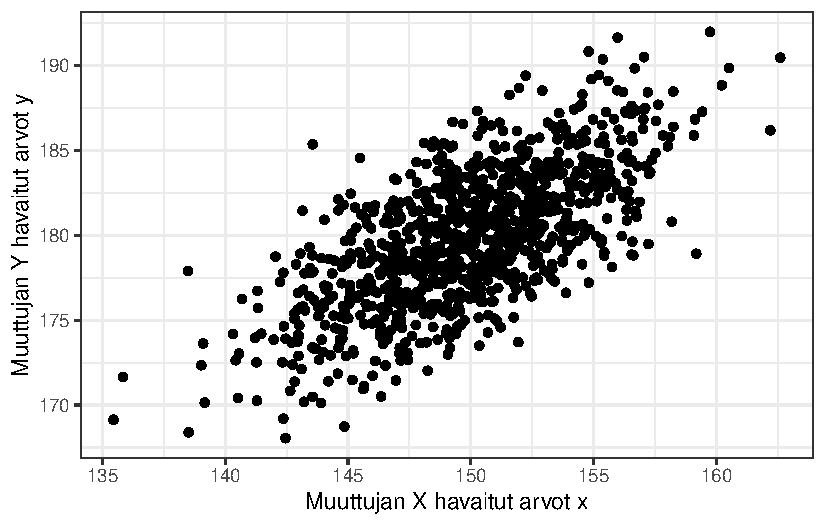
\includegraphics{Tiivistelma6_files/figure-pdf/unnamed-chunk-3-1.pdf}

}

\end{figure}

\hypertarget{satunnaismuuttujien-kovarianssi-ja-korrelaatio}{%
\section{Satunnaismuuttujien kovarianssi ja
korrelaatio}\label{satunnaismuuttujien-kovarianssi-ja-korrelaatio}}

\begin{defblock}{}

\textbf{Satunnaismuuttujien kovarianssi ja korrelaatio}

Olkoon \((X,Y)\) satunnaismuuttujien \(X\) ja \(Y\) muodostama
järjestetty pari. Olkoot \(\mu_X = E(X)\) ja \(\mu_Y = E(Y)\)
satunnaismuuttujien \(X\) ja \(Y\) odotusarvot sekä
\(\sigma^2_X = \text{Var}(X) = E[(X-\mu_X)^2]\) ja
\(\sigma_Y^2 = \text{Var}(Y) = E[(Y-\mu_Y)^2]\) satunnaismuuttujien
\(X\) ja \(Y\) varianssit.

Satunnaismuuttujien \(X\) ja \(Y\) kovarianssi \(\sigma_{XY}\)
määritellään kaavalla

\begin{equation*}

\sigma\_{XY} = \text{Cov}(X,Y) = E\[(X-\\mu_X)(Y-\\mu_Y)\]

\end{equation*}

ja korrelaatio \(\rho_{XY}\) määritellään kaavalla

\begin{equation*}

\rho\_{XY} = \text{Cor}(X,Y) = \frac{\sigma_{XY}}{\sigma_X \sigma_Y}

\end{equation*}

\end{defblock}

\hypertarget{pearsonin-otoskorrelaatiokerroin}{%
\section{Pearsonin
otoskorrelaatiokerroin}\label{pearsonin-otoskorrelaatiokerroin}}

\begin{defblock}{}
\textbf{Pearsonin otoskorrelaatiokerroin}

O

\end{defblock}

\hypertarget{kausaalisuus}{%
\section{Kausaalisuus}\label{kausaalisuus}}



\end{document}
